\documentclass[10pt, a4paper]{article}
\usepackage[paper=a4paper, left=1.5cm, right=1.5cm, bottom=1.5cm, top=2cm]{geometry}
\usepackage[utf8]{inputenc}
\usepackage[T1]{fontenc}
\usepackage[spanish]{babel}
\usepackage{indentfirst}
\usepackage{fancyhdr}
\usepackage{lastpage}
\usepackage{calc}
\usepackage{caratula}
\usepackage{multicol}
% \usepackage{algorithmic}
\usepackage{algorithm}
\usepackage{algorithmicx}
\usepackage{algpseudocode}
\setlength{\columnsep}{1.5cm}
\usepackage{graphicx}
\graphicspath{{imagenes/}}
%\sloppy
\parskip=5pt % 10pt es el tamano de fuente

\usepackage{stringenc}
\usepackage{pdfescape}


\begin{document}

\title{Algo3 - TP1}
\materia{Algoritmos y Estructuras de Datos III}
\submateria{Primer cuatrimestre 2016}
\titulo{Informe}
\subtitulo{RTP1}
\grupo{}

\begin{center}

\includegraphics[width=350pt]{logo}
\end{center}

\integrante{Uriel Jonathan Rozenberg}{848/12}{urielrozenberg@hotmail.com}

\maketitle
\newpage\null\thispagestyle{empty}\newpage
\setcounter{page}{1}
%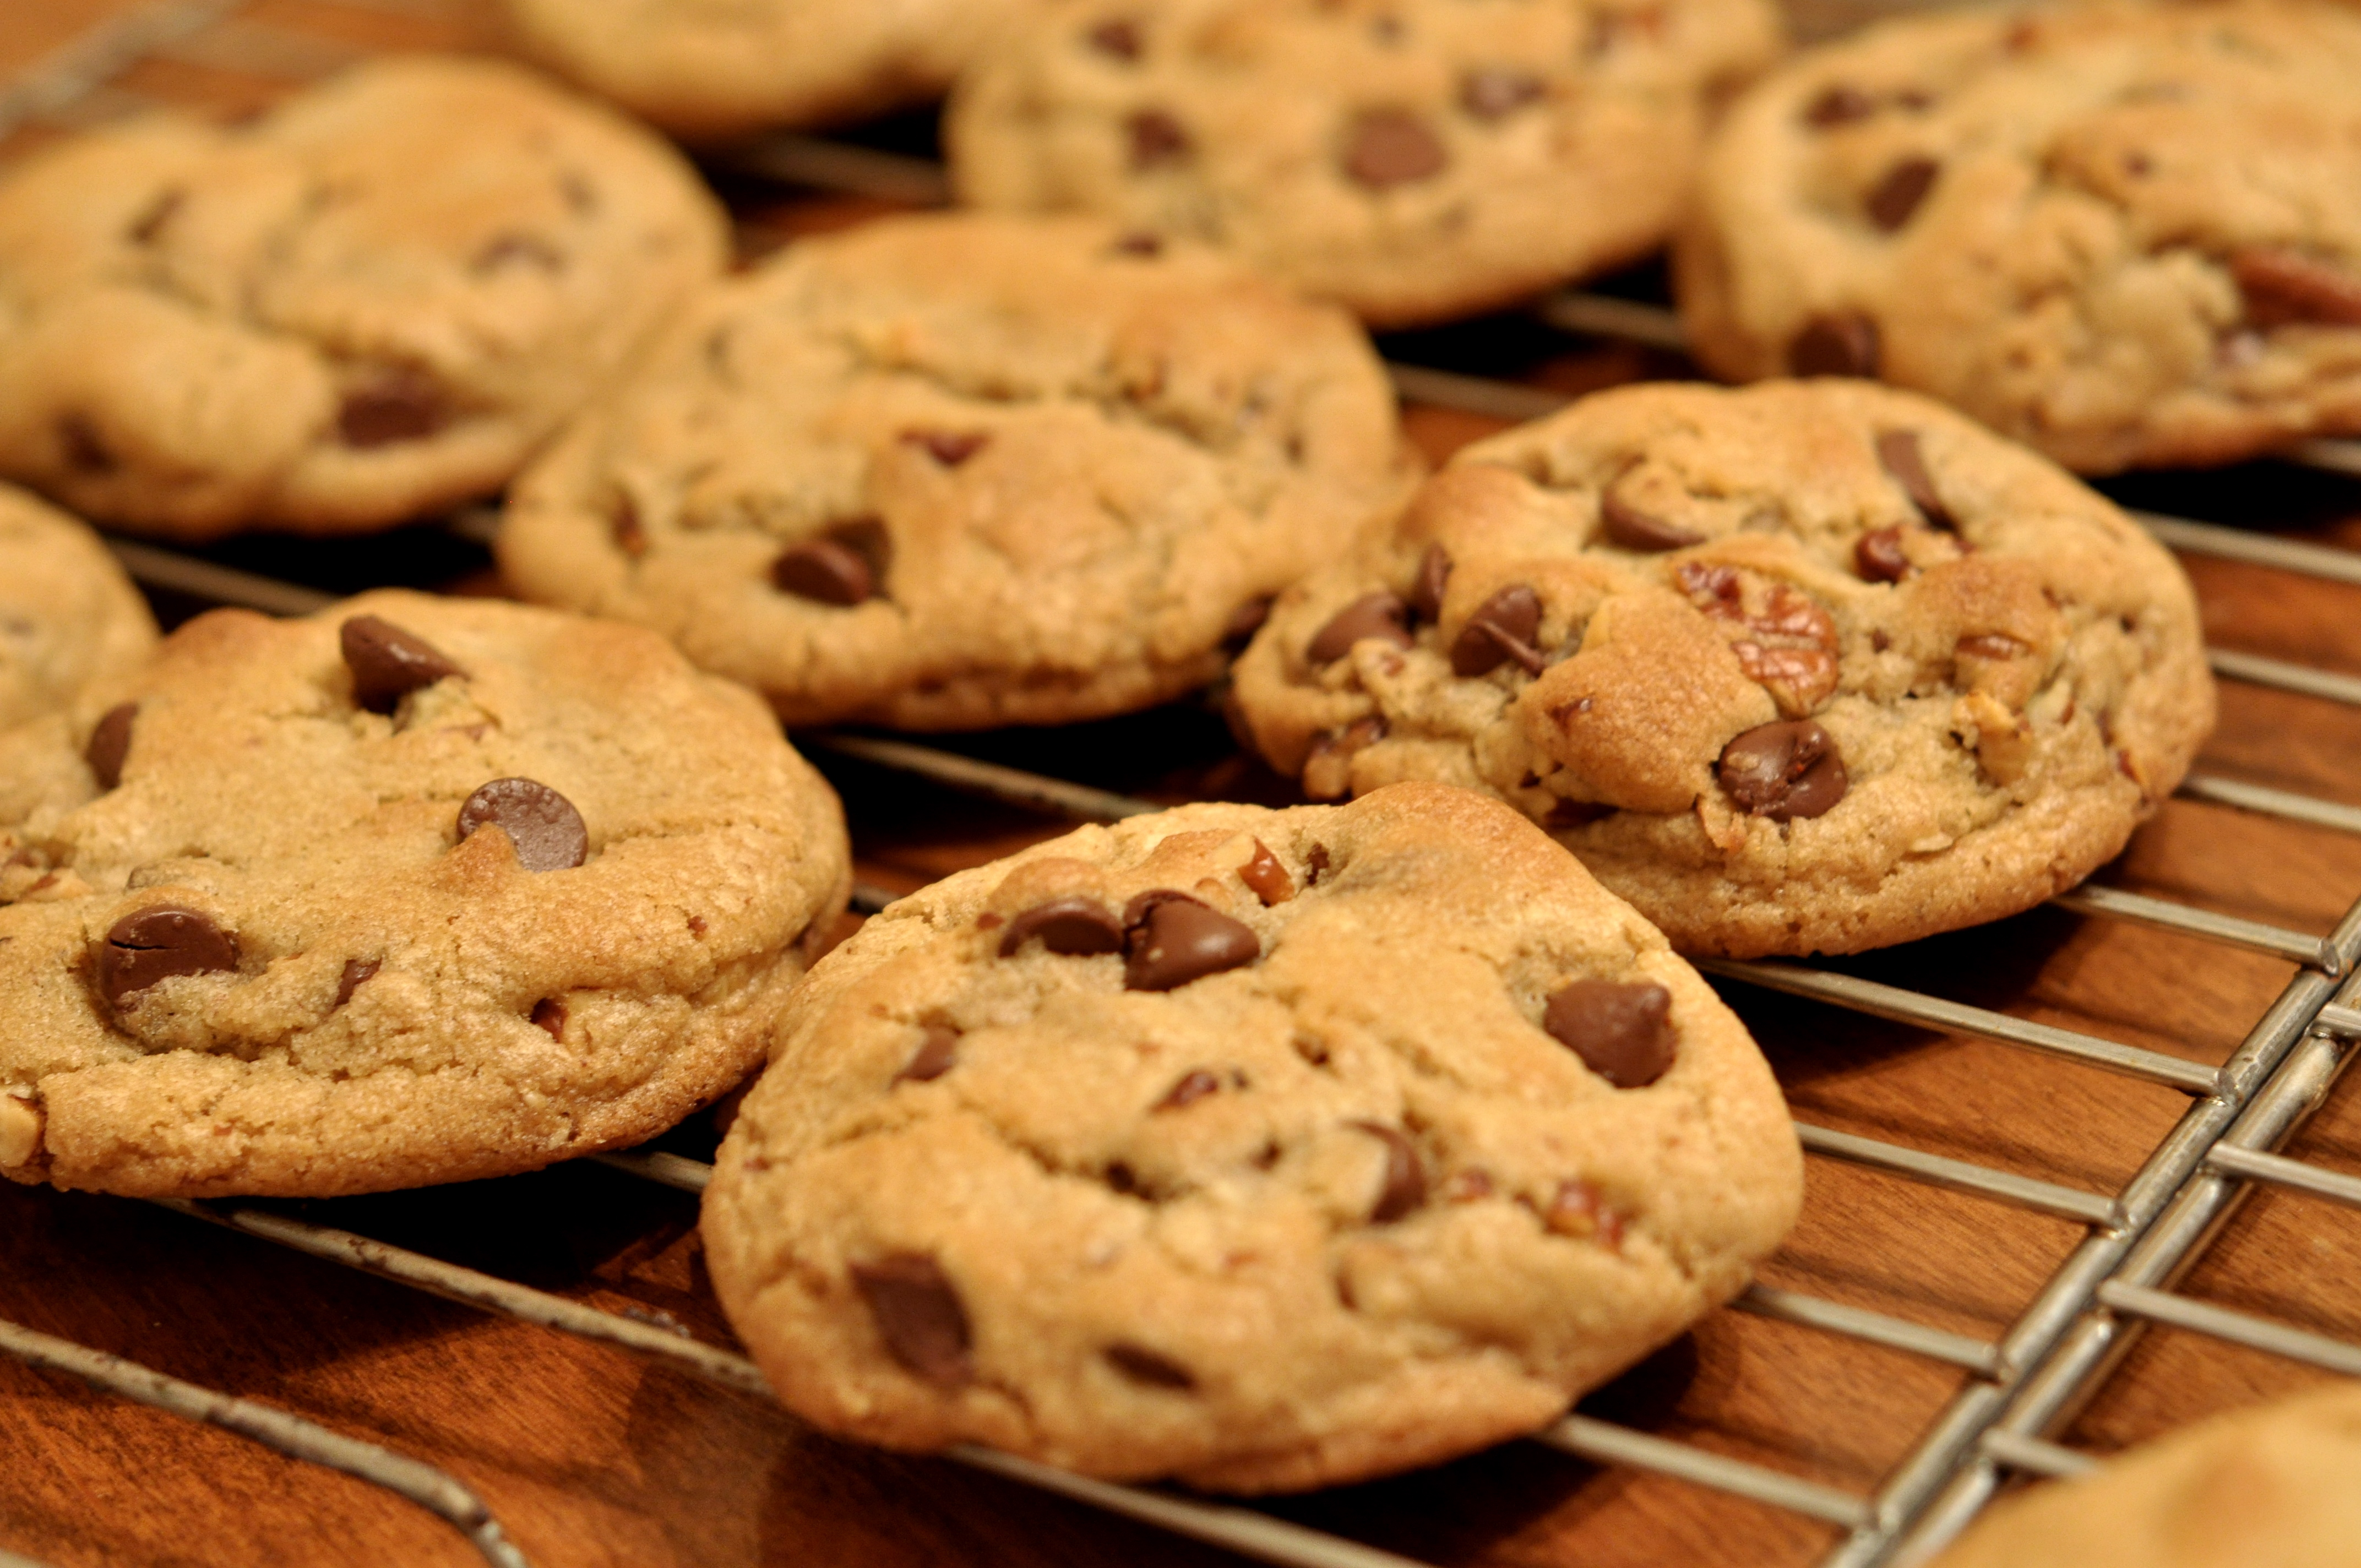
\includegraphics[width=\textwidth]{cookies}  ejemplo para incluir imagenes

\section{Problema 1:  Kaio Ken}
\subsection{Introducción}
\subsubsection{Explicación del problema}
Tenemos un plano del cual no nos importan sus dimensiones. Suponiendo que el plano está inicialmente vacío y la entrada del problema consiste en una serie de posiciones que cumplen $X_1 > X_2 > … > X_n \geq 0$ y $0 \leq Y_1 \leq Y_2 \leq … \leq Y_n$, consideramos que esas posiciones en el plano están ocupadas. Además, hay otro parámetro de entrada, $t \geq 0$.
El problema consiste en buscar el menor número de intentos necesarios para remover las posiciones ocupadas. 

Si uno se “ubica” en una posición dada $(x_0, y_0)$, se remueve ese punto y otros, siguiendo una regla: son aquellos cuyas coordenadas $x$ e $y$ cumplen $0 \leq x \leq x_0 + t$, $0 \leq y \leq y_0 + t$.

Por ejemplo, si tenemos sólo dos puntos de entrada, que cumplen las hipótesis, para los cuales sus coordenadas $x$ e $y$ difieren en 2; y el parámetro $t$ = 1. Entonces la cantidad mínima de intentos es 2, ya que si elegimos el punto 1 no se remueve el 2 y viceversa.

\subsubsection{Ideas}

Sabiendo que tienen que desaparecer todos los puntos, en particular tiene que desaparecer el primero de los que aún estan vivos. Entonces, para matarlo intentamos maximizar la efectividad de la genkidama que tiramos, lo que significa que queremos encontrar la genkidama que mata a más enemigos de entre las que lo matan a él.

Para lograr esto hicimos un algoritmo goloso, que lo que hace es:
\begin{itemize}
\item Me paro en el enemigo que aun este vivo, al que llamaremos $E_1$.
\item Avanzo al siguiente a $E_1$, al que llamaremos $E_2$, me fijo si tirarle la genkidama mata a $E_1$.
\item Si lo mata, me fijo iterativamente si el siguiente de $E_2$, llamado $E_3$, al tirarle la genkidama mata a $E_1$... y así sucesivamente hasta llegar al primer enemigo al que tirarle la genkidama no mate a $E_1$ o bien se acaben los enemigos.
\item Si se encontró un enemigo $E_i$ tal que al tirar la genkidama en su posición $E_1$ no muere, entonces tiramos la genkidama en la posición de $E_{i-1}$. Si para todas las posiciones de los enemigos recorridos se mataba a $E_1$, entonces tiramos la genkidama en el último. En este último caso el algoritmo termina, ya no quedan enemigos vivos.
\item Me paro en $E_i$, y me fijo si la genkidama tirada en $E_{i-1}$ lo alcanza. Si lo alcanza, sigo avanzando hasta que no queden enemigos o bien se encuentre uno, $E_j$, para el cual la genkidama tirada en la posición de $E_{i-1}$ no lo mate. Si la genkidama mataba a todos los enemigos restantes, entonces el algoritmo termina.
\item La genkidama mató a todos los enemigos anteriores a $E_j$, entonces ahora éste es el primer enemigo vivo, y se vuelve al principio.

\end{itemize}
\subsection{Correctitud}
Pseudo pseudo pseudo codigo solucion del problema:

Me paro en el enemigo que aun este vivo, al que llamaremos E1.
Me paro en el siguiente a E1, al que llamaremos E2, me fijo si lo mata a E1.
si lo mata, me fijo iterativamente si el siguiente de E2, llamado E3.. y asi susesivamente hasta llegar al ultimo enemigo que mate a E1 o bien se acaben los enemigos.
para el ultimo enemigo marcado, lo llamamos Ei.
Decinimos que Ei sera donde se tirara la siguiente genkidama.
Me paro en el siguiente enemigo de Ei, lo llamamos Ei+1, y nos fijamos si, tirando la genkidama en Ei, muere tambien E1+1.
luego repetimos el proceso con Ei+2 y asi sucesitvamente hasta llegar al ultimo enemigo que muera al tirar la genkidama en Ei o bien al ultimo enemigo restante y lo llamamos Ej.

y vuelvo al principio si aun quedan enemigos vivos


Para probar la correctitud de este algoritmo hay qur probar dos cosas:
1.que cubre todos los puntos
2.que es el resultado minimo:


1.Esta demostracion seria trivial, es parte del algoritmo  calcular que se cubran todos los puntos fijandose si la ultima genkidama tirada mata hasta un punto y sino, ver desde donde se tiraria la proxima genkidama para que lo mate, para todos los puntos.

2.lo hacemos por induccion sobre la cantidad de puntos.

La hipotesis inductiva es que para N puntos el algoritmo es minimo

Caso base:
numero de puntos = 1:
Esta demostracion es trivial. el algoritmo nos muestra que tira la genkidama en ese unico punto y no se pueden tirar menos genkidamas

Caso N+1:
Dada  la HI, si agregamos un punto mas respetando las condiciones nos quedarian tres casos:
1.O bien la solucion planteada para los N primeros puntos alcanza para que muera el N+1 enemigo, en ese caso seguiria siendo minimo
2.O bien si la genkidama se tiraba en el punto N, y tirarla en N+1 mataria a N, entonces  en vez de tirarse en N se tira en N+1, nuevamente dando minimo
3.O bien el punto esta lo suficientemente lejos del resto de los puntos como para que la unica forma de matar a ese enemigo sea tirandole una genkidama a ese punto y dicha genkidama no mate a nadie, en ese caso volveria a ser un minimo por que se requeriria si o si una genkidama mas para llegar a ese punto
\subsection{Complejidad}
\newpage
\subsubsection{Pseudocódigo}
\begin{algorithm}
\caption{Estructura del algoritmo de D\&C}
\begin{algorithmic}[1]
	\Function{D\&C}{}
	\State{\textbf{Int} $rango$ := $[log_2(N)]$}
	\For{$i$ := $1$ hasta $rango$}
		\For{$x$ := $0$ hasta $N$}
        \If{$x$ mod $2*i < 2*(i-1)$}
            \State{Imprimir “1”}
        \Else
        	\State{Imprimir “2”}
        \EndIf
        \State{$x++$}
        \EndFor
    \State{$i++$} 
	\EndFor
	\EndFunction
\end{algorithmic}
\end{algorithm}
%este deberia ser el post
% Int rango := log2(n) + 2
% If (n == 2(rango -2 )) rango := rango - 1
% Para i := 1 hasta rango hacer
% 	Para x := 0 hasta n hacer
% 		Si x mod 2i < 2(i – 1) entonces 
% Imprimir “1”
% 		Else aw
% Imprimir “2”
% 		Fin Si
% 		X++
% 	Fin Para
% 	I++
% Fin Para

\subsubsection{Análisis} 
%EL corrector dijo que esto estaba bien, si demostraba bien la correctitud, pero no se si hace falta mas  explicacion
El algoritmo hace dos ciclos anidados. El primero lo hace $log_2(N)$ veces y el otro $N$ veces, mientras que todas las operaciones adentro de ambos ciclos tienen costo de $O(1)$ dando una complejidad final de $O(NLog(N))$.
\subsection{Análisis experimental}
En este caso los parámetros de entrada son el vector de enemigos y el $t$, por lo tanto experimentamos variando las distribuciones y $t$.

% \subsubsection{Mediciones para el comportamiento del caso promedio}

% %TODO no tenia idea de que mediciones usar, voy a decir fruta pero falta el grafico
% Se realizaron mediciones para el mejor, peor y caso promedio. Las mediciones se realizaron usando ... %como es t, N, la distribucion?
% Se obtuvieron los siguientes gráficos:

% \begin{figure}[h!]
% % \includegraphics[width=\textwidth]{p2_1}
% \caption{Gráfico obtenido a partir de las mediciones realizadas en el problema 2}
% \end{figure}

% Se puede observar un comportamiento lineal en las mediciones obtenidas, tal y como se esperaba del cálculo de complejidad.

\subsubsection{Mediciones con $t$ constante y $N$ variable}

Se realizaron mediciones para distribuciones aleatorias con $N$ = 2000 de diferentes valores de $t$: 1, 10, 100 y 1000. Las distribuciones aleatorias para cada $1 \leq n \leq N$ se hicieron con valores entre 0 y $n$ tanto en $x$ como en $y$, de forma tal de mantener constante el promedio de densidad de puntos (que se traduce en una separación aproximada de 1 entre coordenadas de puntos contiguos). De esta forma se pueden comparar entre sí. Se obtuvieron los siguientes gráficos:

\begin{figure}[h!]
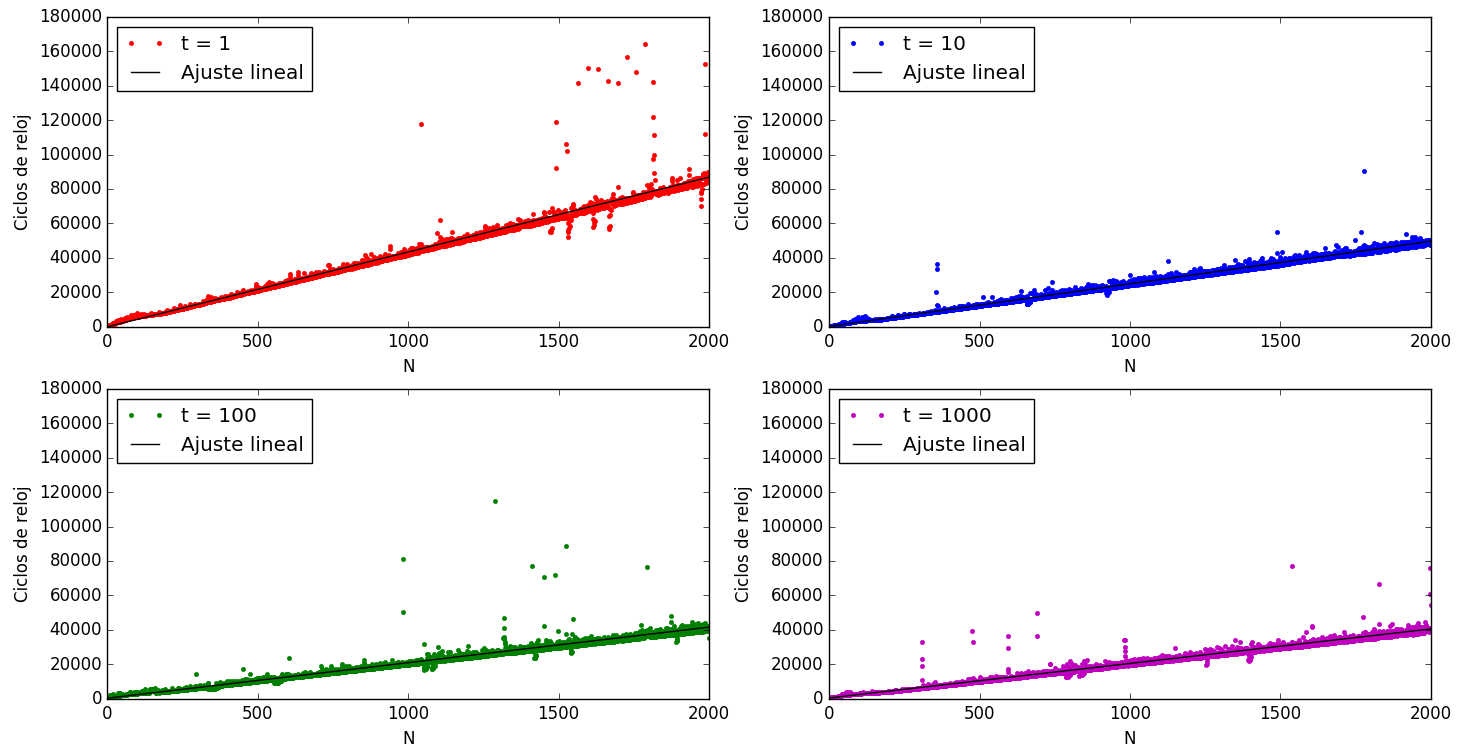
\includegraphics[width=\textwidth]{p2_2_1}
\caption{Gráfico obtenido a partir de las mediciones realizadas diferentes valores de $t$ en el problema 2}
\end{figure}

\begin{figure}[h!]
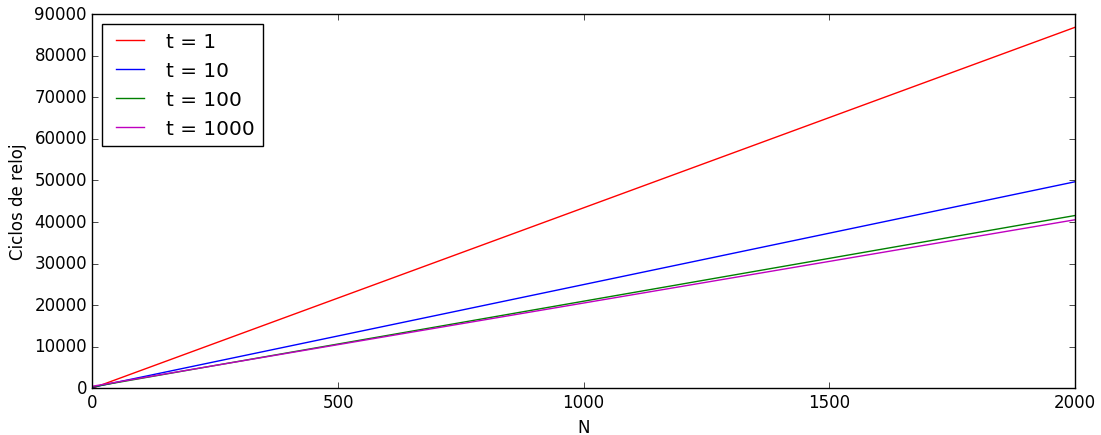
\includegraphics[width=\textwidth]{p2_2_2}
\caption{Comparación entre los ajustes lineales para los diferentes valores de $t$}
\end{figure}

En todos los casos se pudo ajustar satisfactoriamente con una función lineal, como esperábamos a causa de que la complejidad es lineal para todos los casos.

Se observa que cuanto mayor es el valor de $t$, menor es la cantidad de ciclos de reloj necesarias. Esto es así ya que cada una de las genkidamas tiene un rango mayor, lo que resulta en más enemigos muertos por genkidama en promedio. Además se puede observar que el caso con $t$ = 1 está cerca del peor caso (casi 1 $N$ genkidamas) mientras que el caso con $t$ = 1000 está cerca del mejor caso (casi 1 genkidama en total).

\begin{multicols}{2}
Comparando los valores de pendientes ajustadas y el segundo gráfico se puede ver que la pendiente decrece rápidamente al principio, llegando a alcanzar la mitad de su valor. Esto es consistente con la diferencia en complejidad entre el mejor y el peor caso, que es $O(N)$ y $O(2N)$ respectivamente.

\begin{description}
\item[Pendiente para t = 1] $\approx43,416$
\item[Pendiente para t = 10] $\approx24,727$
\item[Pendiente para t = 100] $\approx20,608$
\item[Pendiente para t = 1000] $\approx20,026$
\end{description}
\end{multicols}
%TODO : no es consistente porque antes decia 3N(lo cambie). no se cual poner u,u

\subsubsection{Mediciones con distribución constante y $t$ variable}

Se realizaron mediciones usando siempre la misma distribución generada aleatoriamente con $N$ = 2000 elementos. La separación promedio $d$ entre las coordenadas de los puntos para un caso fue 100, para otro 500 y para otro 1000. Se varió $t$ entre 1 y 2000 y se obtuvieron los siguientes resultados:

\begin{figure}[h!]
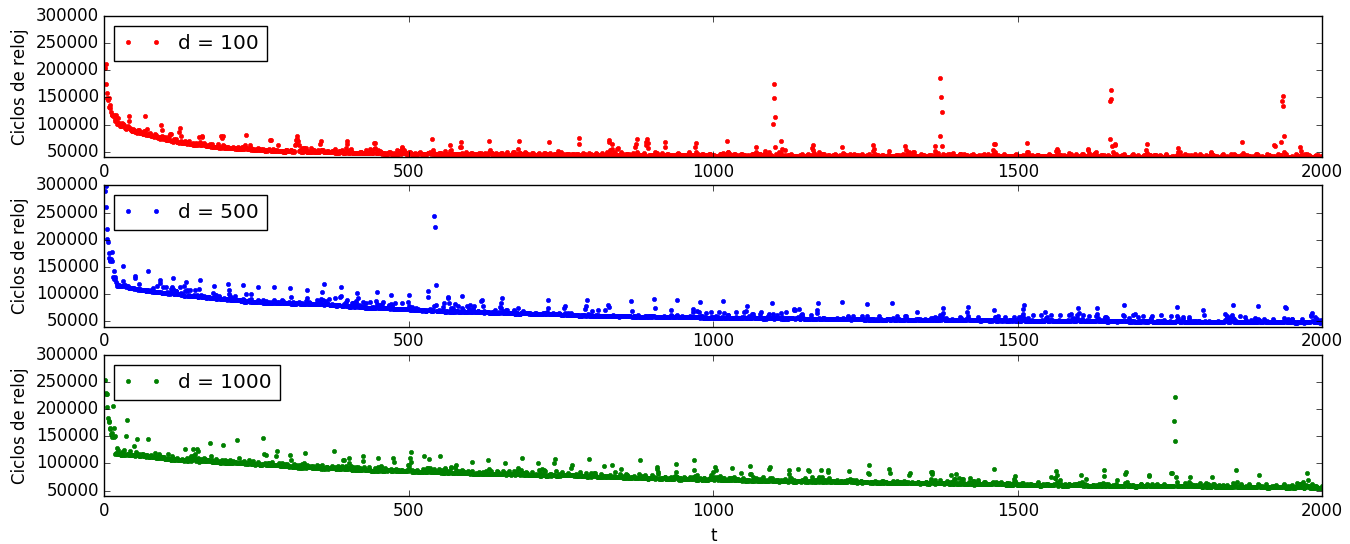
\includegraphics[width=\textwidth]{p2_3}
\caption{Mediciones para $t$ variable y distribución fija con distintas separaciones promedio entre puntos}
\end{figure}

Se observa en todos los casos que cerca de $t$ = 0 la cantidad de ciclos de reloj es alta y desciende abruptamente. También se puede ver que en el caso de los puntos más juntos, se llega al tiempo mínimo (la cota inferior de la cantidad de ciclos de reloj) antes que en los otros dos casos. Esto tiene sentido puesto que el mejor caso debería encontrarse antes cuanto más juntos estén los puntos, cuando $t \approx d$. Y se observa efectivamente que es en esa parte del gráfico en la cual se llega a la asíntota.


\section{Problema 2:  Genkidama}
\subsection{Introducción}
\subsubsection{Explicación del problema}
Tenemos un plano del cual no nos importan sus dimensiones. Suponiendo que el plano está inicialmente vacío y la entrada del problema consiste en una serie de posiciones que cumplen $X_1 > X_2 > … > X_n \geq 0$ y $0 \leq Y_1 \leq Y_2 \leq … \leq Y_n$, consideramos que esas posiciones en el plano están ocupadas. Además, hay otro parámetro de entrada, $t \geq 0$.
El problema consiste en buscar el menor número de intentos necesarios para remover las posiciones ocupadas. 

Si uno se “ubica” en una posición dada $(x_0, y_0)$, se remueve ese punto y otros, siguiendo una regla: son aquellos cuyas coordenadas $x$ e $y$ cumplen $0 \leq x \leq x_0 + t$, $0 \leq y \leq y_0 + t$.

Por ejemplo, si tenemos sólo dos puntos de entrada, que cumplen las hipótesis, para los cuales sus coordenadas $x$ e $y$ difieren en 2; y el parámetro $t$ = 1. Entonces la cantidad mínima de intentos es 2, ya que si elegimos el punto 1 no se remueve el 2 y viceversa.

\subsubsection{Ideas}

Sabiendo que tienen que desaparecer todos los puntos, en particular tiene que desaparecer el primero de los que aún estan vivos. Entonces, para matarlo intentamos maximizar la efectividad de la genkidama que tiramos, lo que significa que queremos encontrar la genkidama que mata a más enemigos de entre las que lo matan a él.

Para lograr esto hicimos un algoritmo goloso, que lo que hace es:
\begin{itemize}
\item Me paro en el enemigo que aun este vivo, al que llamaremos $E_1$.
\item Avanzo al siguiente a $E_1$, al que llamaremos $E_2$, me fijo si tirarle la genkidama mata a $E_1$.
\item Si lo mata, me fijo iterativamente si el siguiente de $E_2$, llamado $E_3$, al tirarle la genkidama mata a $E_1$... y así sucesivamente hasta llegar al primer enemigo al que tirarle la genkidama no mate a $E_1$ o bien se acaben los enemigos.
\item Si se encontró un enemigo $E_i$ tal que al tirar la genkidama en su posición $E_1$ no muere, entonces tiramos la genkidama en la posición de $E_{i-1}$. Si para todas las posiciones de los enemigos recorridos se mataba a $E_1$, entonces tiramos la genkidama en el último. En este último caso el algoritmo termina, ya no quedan enemigos vivos.
\item Me paro en $E_i$, y me fijo si la genkidama tirada en $E_{i-1}$ lo alcanza. Si lo alcanza, sigo avanzando hasta que no queden enemigos o bien se encuentre uno, $E_j$, para el cual la genkidama tirada en la posición de $E_{i-1}$ no lo mate. Si la genkidama mataba a todos los enemigos restantes, entonces el algoritmo termina.
\item La genkidama mató a todos los enemigos anteriores a $E_j$, entonces ahora éste es el primer enemigo vivo, y se vuelve al principio.

\end{itemize}
\subsection{Correctitud}
Pseudo pseudo pseudo codigo solucion del problema:

Me paro en el enemigo que aun este vivo, al que llamaremos E1.
Me paro en el siguiente a E1, al que llamaremos E2, me fijo si lo mata a E1.
si lo mata, me fijo iterativamente si el siguiente de E2, llamado E3.. y asi susesivamente hasta llegar al ultimo enemigo que mate a E1 o bien se acaben los enemigos.
para el ultimo enemigo marcado, lo llamamos Ei.
Decinimos que Ei sera donde se tirara la siguiente genkidama.
Me paro en el siguiente enemigo de Ei, lo llamamos Ei+1, y nos fijamos si, tirando la genkidama en Ei, muere tambien E1+1.
luego repetimos el proceso con Ei+2 y asi sucesitvamente hasta llegar al ultimo enemigo que muera al tirar la genkidama en Ei o bien al ultimo enemigo restante y lo llamamos Ej.

y vuelvo al principio si aun quedan enemigos vivos


Para probar la correctitud de este algoritmo hay qur probar dos cosas:
1.que cubre todos los puntos
2.que es el resultado minimo:


1.Esta demostracion seria trivial, es parte del algoritmo  calcular que se cubran todos los puntos fijandose si la ultima genkidama tirada mata hasta un punto y sino, ver desde donde se tiraria la proxima genkidama para que lo mate, para todos los puntos.

2.lo hacemos por induccion sobre la cantidad de puntos.

La hipotesis inductiva es que para N puntos el algoritmo es minimo

Caso base:
numero de puntos = 1:
Esta demostracion es trivial. el algoritmo nos muestra que tira la genkidama en ese unico punto y no se pueden tirar menos genkidamas

Caso N+1:
Dada  la HI, si agregamos un punto mas respetando las condiciones nos quedarian tres casos:
1.O bien la solucion planteada para los N primeros puntos alcanza para que muera el N+1 enemigo, en ese caso seguiria siendo minimo
2.O bien si la genkidama se tiraba en el punto N, y tirarla en N+1 mataria a N, entonces  en vez de tirarse en N se tira en N+1, nuevamente dando minimo
3.O bien el punto esta lo suficientemente lejos del resto de los puntos como para que la unica forma de matar a ese enemigo sea tirandole una genkidama a ese punto y dicha genkidama no mate a nadie, en ese caso volveria a ser un minimo por que se requeriria si o si una genkidama mas para llegar a ese punto
\subsection{Complejidad}
\newpage
\subsubsection{Pseudocódigo}
\begin{algorithm}
\caption{Estructura del algoritmo de D\&C}
\begin{algorithmic}[1]
	\Function{D\&C}{}
	\State{\textbf{Int} $rango$ := $[log_2(N)]$}
	\For{$i$ := $1$ hasta $rango$}
		\For{$x$ := $0$ hasta $N$}
        \If{$x$ mod $2*i < 2*(i-1)$}
            \State{Imprimir “1”}
        \Else
        	\State{Imprimir “2”}
        \EndIf
        \State{$x++$}
        \EndFor
    \State{$i++$} 
	\EndFor
	\EndFunction
\end{algorithmic}
\end{algorithm}
%este deberia ser el post
% Int rango := log2(n) + 2
% If (n == 2(rango -2 )) rango := rango - 1
% Para i := 1 hasta rango hacer
% 	Para x := 0 hasta n hacer
% 		Si x mod 2i < 2(i – 1) entonces 
% Imprimir “1”
% 		Else aw
% Imprimir “2”
% 		Fin Si
% 		X++
% 	Fin Para
% 	I++
% Fin Para

\subsubsection{Análisis} 
%EL corrector dijo que esto estaba bien, si demostraba bien la correctitud, pero no se si hace falta mas  explicacion
El algoritmo hace dos ciclos anidados. El primero lo hace $log_2(N)$ veces y el otro $N$ veces, mientras que todas las operaciones adentro de ambos ciclos tienen costo de $O(1)$ dando una complejidad final de $O(NLog(N))$.
\subsection{Analisis experimental}
En este caso los parámetros de entrada son el vector de enemigos y el $t$, por lo tanto experimentamos variando las distribuciones y $t$.

% \subsubsection{Mediciones para el comportamiento del caso promedio}

% %TODO no tenia idea de que mediciones usar, voy a decir fruta pero falta el grafico
% Se realizaron mediciones para el mejor, peor y caso promedio. Las mediciones se realizaron usando ... %como es t, N, la distribucion?
% Se obtuvieron los siguientes gráficos:

% \begin{figure}[h!]
% % \includegraphics[width=\textwidth]{p2_1}
% \caption{Gráfico obtenido a partir de las mediciones realizadas en el problema 2}
% \end{figure}

% Se puede observar un comportamiento lineal en las mediciones obtenidas, tal y como se esperaba del cálculo de complejidad.

\subsubsection{Mediciones con $t$ constante y $N$ variable}

Se realizaron mediciones para distribuciones aleatorias con $N$ = 2000 de diferentes valores de $t$: 1, 10, 100 y 1000. Las distribuciones aleatorias para cada $1 \leq n \leq N$ se hicieron con valores entre 0 y $n$ tanto en $x$ como en $y$, de forma tal de mantener constante el promedio de densidad de puntos (que se traduce en una separación aproximada de 1 entre coordenadas de puntos contiguos). De esta forma se pueden comparar entre sí. Se obtuvieron los siguientes gráficos:

\begin{figure}[h!]
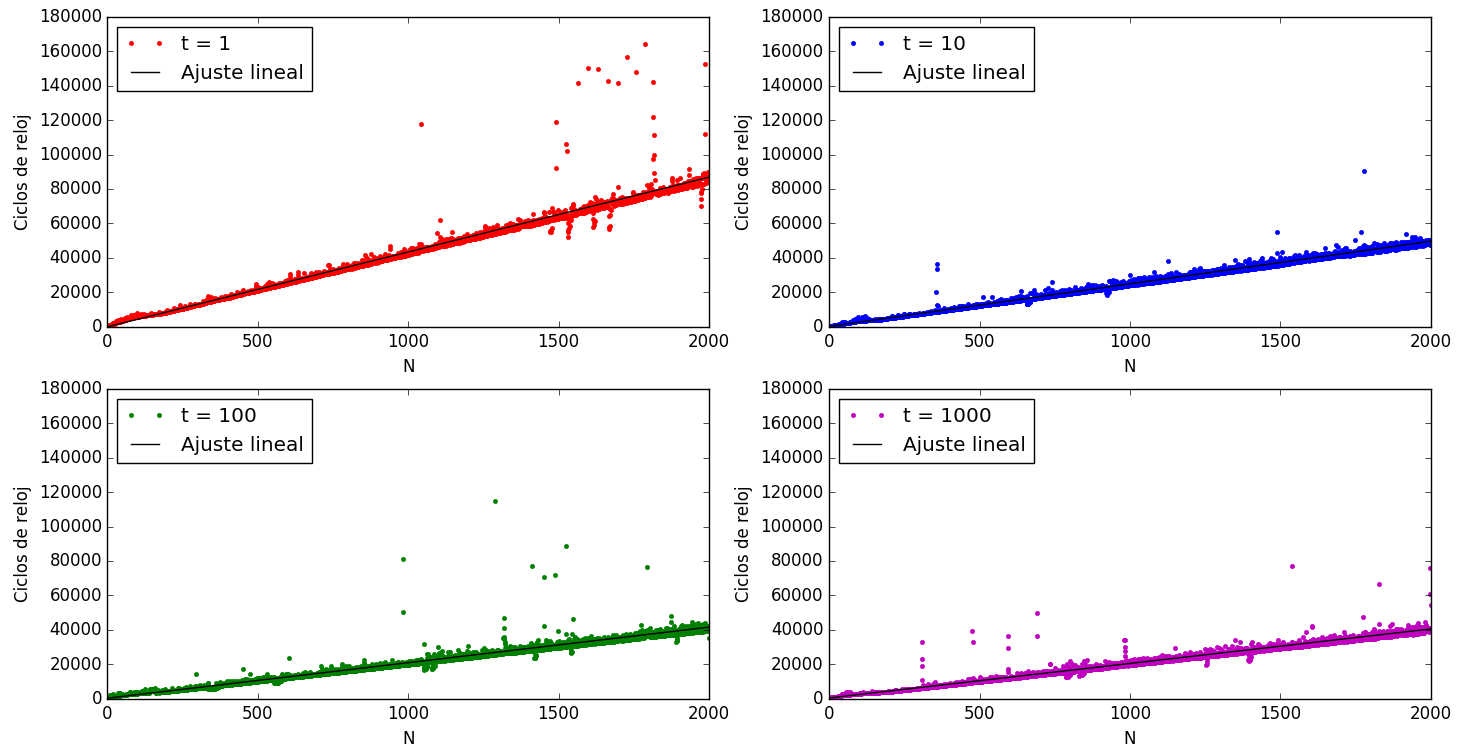
\includegraphics[width=\textwidth]{p2_2_1}
\caption{Gráfico obtenido a partir de las mediciones realizadas diferentes valores de $t$ en el problema 2}
\end{figure}

\begin{figure}[h!]
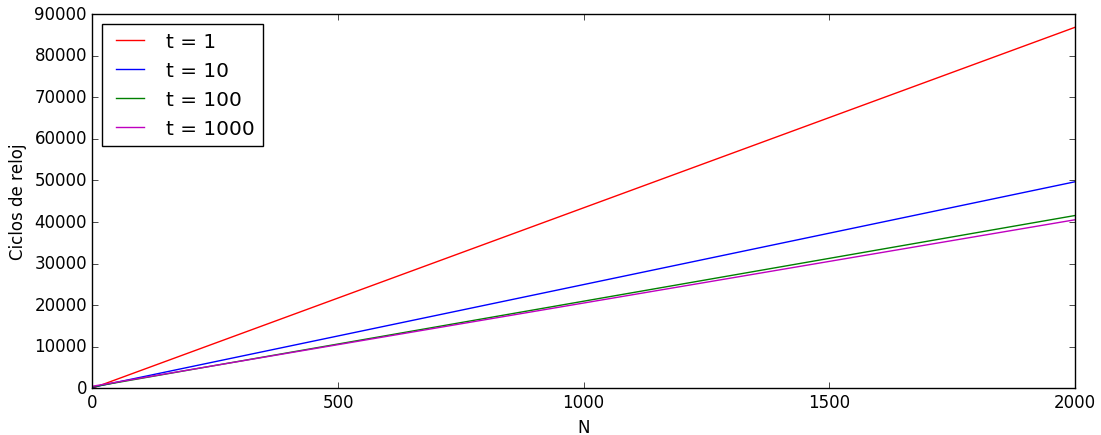
\includegraphics[width=\textwidth]{p2_2_2}
\caption{Comparación entre los ajustes lineales para los diferentes valores de $t$}
\end{figure}

En todos los casos se pudo ajustar satisfactoriamente con una función lineal, como esperábamos a causa de que la complejidad es lineal para todos los casos.

Se observa que cuanto mayor es el valor de $t$, menor es la cantidad de ciclos de reloj necesarias. Esto es así ya que cada una de las genkidamas tiene un rango mayor, lo que resulta en más enemigos muertos por genkidama en promedio. Además se puede observar que el caso con $t$ = 1 está cerca del peor caso (casi 1 $N$ genkidamas) mientras que el caso con $t$ = 1000 está cerca del mejor caso (casi 1 genkidama en total).

\begin{multicols}{2}
Comparando los valores de pendientes ajustadas y el segundo gráfico se puede ver que la pendiente decrece rápidamente al principio, llegando a alcanzar la mitad de su valor. Esto es consistente con la diferencia en complejidad entre el mejor y el peor caso, que es $O(N)$ y $O(2N)$ respectivamente.

\begin{description}
\item[Pendiente para t = 1] $\approx43,416$
\item[Pendiente para t = 10] $\approx24,727$
\item[Pendiente para t = 100] $\approx20,608$
\item[Pendiente para t = 1000] $\approx20,026$
\end{description}
\end{multicols}
%TODO : no es consistente porque antes decia 3N(lo cambie). no se cual poner u,u

\subsubsection{Mediciones con distribución constante y $t$ variable}

Se realizaron mediciones usando siempre la misma distribución generada aleatoriamente con $N$ = 2000 elementos. La separación promedio $d$ entre las coordenadas de los puntos para un caso fue 100, para otro 500 y para otro 1000. Se varió $t$ entre 1 y 2000 y se obtuvieron los siguientes resultados:

\begin{figure}[h!]
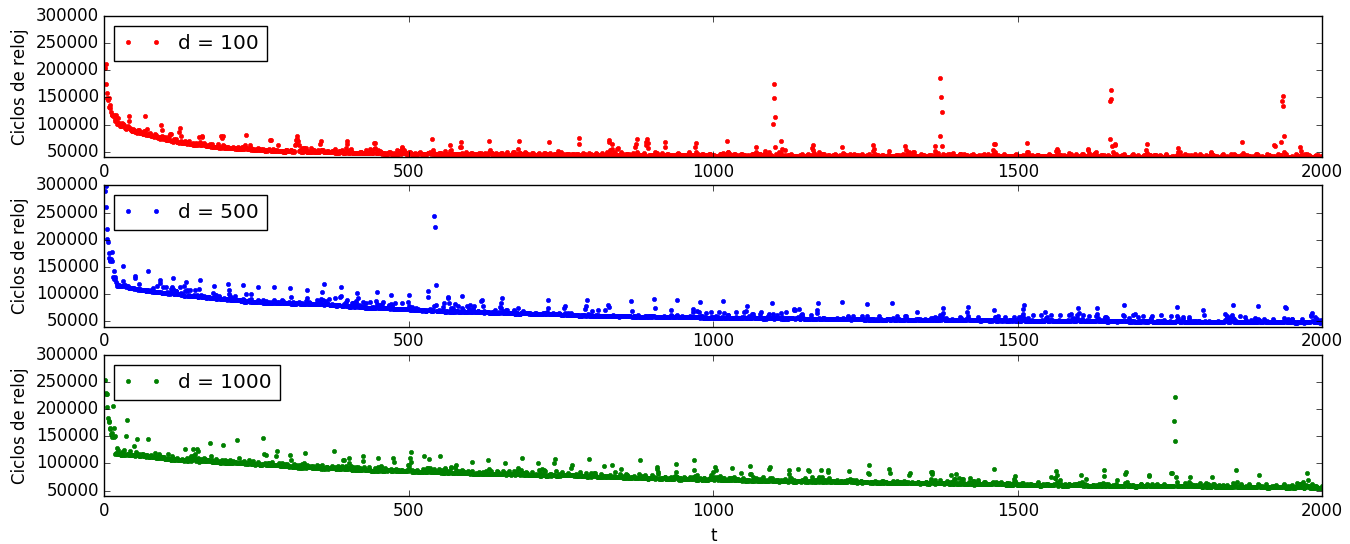
\includegraphics[width=\textwidth]{p2_3}
\caption{Mediciones para $t$ variable y distribución fija con distintas separaciones promedio entre puntos}
\end{figure}

Se observa en todos los casos que cerca de $t$ = 0 la cantidad de ciclos de reloj es alta y desciende abruptamente. También se puede ver que en el caso de los puntos más juntos, se llega al tiempo mínimo (la cota inferior de la cantidad de ciclos de reloj) antes que en los otros dos casos. Esto tiene sentido puesto que el mejor caso debería encontrarse antes cuanto más juntos estén los puntos, cuando $t \approx d$. Y se observa efectivamente que es en esa parte del gráfico en la cual se llega a la asíntota.


\section{Problema 3: Kamehameha}
\subsection{Introducción}
\subsubsection{Explicación del problema}
Tenemos un plano del cual no nos importan sus dimensiones. Suponiendo que el plano está inicialmente vacío y la entrada del problema consiste en una serie de posiciones que cumplen $X_1 > X_2 > … > X_n \geq 0$ y $0 \leq Y_1 \leq Y_2 \leq … \leq Y_n$, consideramos que esas posiciones en el plano están ocupadas. Además, hay otro parámetro de entrada, $t \geq 0$.
El problema consiste en buscar el menor número de intentos necesarios para remover las posiciones ocupadas. 

Si uno se “ubica” en una posición dada $(x_0, y_0)$, se remueve ese punto y otros, siguiendo una regla: son aquellos cuyas coordenadas $x$ e $y$ cumplen $0 \leq x \leq x_0 + t$, $0 \leq y \leq y_0 + t$.

Por ejemplo, si tenemos sólo dos puntos de entrada, que cumplen las hipótesis, para los cuales sus coordenadas $x$ e $y$ difieren en 2; y el parámetro $t$ = 1. Entonces la cantidad mínima de intentos es 2, ya que si elegimos el punto 1 no se remueve el 2 y viceversa.

\subsubsection{Ideas}

Sabiendo que tienen que desaparecer todos los puntos, en particular tiene que desaparecer el primero de los que aún estan vivos. Entonces, para matarlo intentamos maximizar la efectividad de la genkidama que tiramos, lo que significa que queremos encontrar la genkidama que mata a más enemigos de entre las que lo matan a él.

Para lograr esto hicimos un algoritmo goloso, que lo que hace es:
\begin{itemize}
\item Me paro en el enemigo que aun este vivo, al que llamaremos $E_1$.
\item Avanzo al siguiente a $E_1$, al que llamaremos $E_2$, me fijo si tirarle la genkidama mata a $E_1$.
\item Si lo mata, me fijo iterativamente si el siguiente de $E_2$, llamado $E_3$, al tirarle la genkidama mata a $E_1$... y así sucesivamente hasta llegar al primer enemigo al que tirarle la genkidama no mate a $E_1$ o bien se acaben los enemigos.
\item Si se encontró un enemigo $E_i$ tal que al tirar la genkidama en su posición $E_1$ no muere, entonces tiramos la genkidama en la posición de $E_{i-1}$. Si para todas las posiciones de los enemigos recorridos se mataba a $E_1$, entonces tiramos la genkidama en el último. En este último caso el algoritmo termina, ya no quedan enemigos vivos.
\item Me paro en $E_i$, y me fijo si la genkidama tirada en $E_{i-1}$ lo alcanza. Si lo alcanza, sigo avanzando hasta que no queden enemigos o bien se encuentre uno, $E_j$, para el cual la genkidama tirada en la posición de $E_{i-1}$ no lo mate. Si la genkidama mataba a todos los enemigos restantes, entonces el algoritmo termina.
\item La genkidama mató a todos los enemigos anteriores a $E_j$, entonces ahora éste es el primer enemigo vivo, y se vuelve al principio.

\end{itemize}
\subsection{Correctitud}
Pseudo pseudo pseudo codigo solucion del problema:

Me paro en el enemigo que aun este vivo, al que llamaremos E1.
Me paro en el siguiente a E1, al que llamaremos E2, me fijo si lo mata a E1.
si lo mata, me fijo iterativamente si el siguiente de E2, llamado E3.. y asi susesivamente hasta llegar al ultimo enemigo que mate a E1 o bien se acaben los enemigos.
para el ultimo enemigo marcado, lo llamamos Ei.
Decinimos que Ei sera donde se tirara la siguiente genkidama.
Me paro en el siguiente enemigo de Ei, lo llamamos Ei+1, y nos fijamos si, tirando la genkidama en Ei, muere tambien E1+1.
luego repetimos el proceso con Ei+2 y asi sucesitvamente hasta llegar al ultimo enemigo que muera al tirar la genkidama en Ei o bien al ultimo enemigo restante y lo llamamos Ej.

y vuelvo al principio si aun quedan enemigos vivos


Para probar la correctitud de este algoritmo hay qur probar dos cosas:
1.que cubre todos los puntos
2.que es el resultado minimo:


1.Esta demostracion seria trivial, es parte del algoritmo  calcular que se cubran todos los puntos fijandose si la ultima genkidama tirada mata hasta un punto y sino, ver desde donde se tiraria la proxima genkidama para que lo mate, para todos los puntos.

2.lo hacemos por induccion sobre la cantidad de puntos.

La hipotesis inductiva es que para N puntos el algoritmo es minimo

Caso base:
numero de puntos = 1:
Esta demostracion es trivial. el algoritmo nos muestra que tira la genkidama en ese unico punto y no se pueden tirar menos genkidamas

Caso N+1:
Dada  la HI, si agregamos un punto mas respetando las condiciones nos quedarian tres casos:
1.O bien la solucion planteada para los N primeros puntos alcanza para que muera el N+1 enemigo, en ese caso seguiria siendo minimo
2.O bien si la genkidama se tiraba en el punto N, y tirarla en N+1 mataria a N, entonces  en vez de tirarse en N se tira en N+1, nuevamente dando minimo
3.O bien el punto esta lo suficientemente lejos del resto de los puntos como para que la unica forma de matar a ese enemigo sea tirandole una genkidama a ese punto y dicha genkidama no mate a nadie, en ese caso volveria a ser un minimo por que se requeriria si o si una genkidama mas para llegar a ese punto
\subsection{Complejidad}
\newpage
\subsubsection{Pseudocódigo}
\begin{algorithm}
\caption{Estructura del algoritmo de D\&C}
\begin{algorithmic}[1]
	\Function{D\&C}{}
	\State{\textbf{Int} $rango$ := $[log_2(N)]$}
	\For{$i$ := $1$ hasta $rango$}
		\For{$x$ := $0$ hasta $N$}
        \If{$x$ mod $2*i < 2*(i-1)$}
            \State{Imprimir “1”}
        \Else
        	\State{Imprimir “2”}
        \EndIf
        \State{$x++$}
        \EndFor
    \State{$i++$} 
	\EndFor
	\EndFunction
\end{algorithmic}
\end{algorithm}
%este deberia ser el post
% Int rango := log2(n) + 2
% If (n == 2(rango -2 )) rango := rango - 1
% Para i := 1 hasta rango hacer
% 	Para x := 0 hasta n hacer
% 		Si x mod 2i < 2(i – 1) entonces 
% Imprimir “1”
% 		Else aw
% Imprimir “2”
% 		Fin Si
% 		X++
% 	Fin Para
% 	I++
% Fin Para

\subsubsection{Análisis} 
%EL corrector dijo que esto estaba bien, si demostraba bien la correctitud, pero no se si hace falta mas  explicacion
El algoritmo hace dos ciclos anidados. El primero lo hace $log_2(N)$ veces y el otro $N$ veces, mientras que todas las operaciones adentro de ambos ciclos tienen costo de $O(1)$ dando una complejidad final de $O(NLog(N))$.
\subsection{Analisis experimental}
En este caso los parámetros de entrada son el vector de enemigos y el $t$, por lo tanto experimentamos variando las distribuciones y $t$.

% \subsubsection{Mediciones para el comportamiento del caso promedio}

% %TODO no tenia idea de que mediciones usar, voy a decir fruta pero falta el grafico
% Se realizaron mediciones para el mejor, peor y caso promedio. Las mediciones se realizaron usando ... %como es t, N, la distribucion?
% Se obtuvieron los siguientes gráficos:

% \begin{figure}[h!]
% % \includegraphics[width=\textwidth]{p2_1}
% \caption{Gráfico obtenido a partir de las mediciones realizadas en el problema 2}
% \end{figure}

% Se puede observar un comportamiento lineal en las mediciones obtenidas, tal y como se esperaba del cálculo de complejidad.

\subsubsection{Mediciones con $t$ constante y $N$ variable}

Se realizaron mediciones para distribuciones aleatorias con $N$ = 2000 de diferentes valores de $t$: 1, 10, 100 y 1000. Las distribuciones aleatorias para cada $1 \leq n \leq N$ se hicieron con valores entre 0 y $n$ tanto en $x$ como en $y$, de forma tal de mantener constante el promedio de densidad de puntos (que se traduce en una separación aproximada de 1 entre coordenadas de puntos contiguos). De esta forma se pueden comparar entre sí. Se obtuvieron los siguientes gráficos:

\begin{figure}[h!]
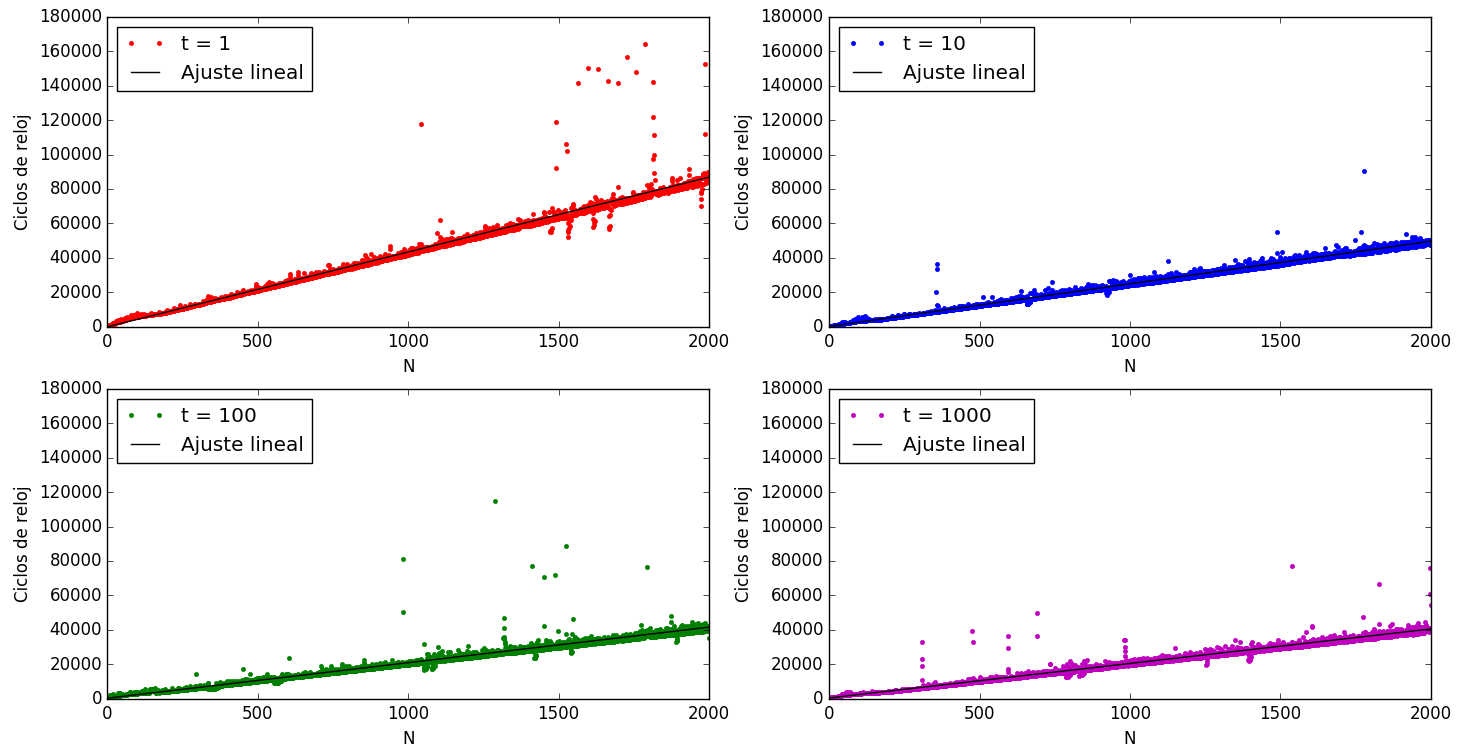
\includegraphics[width=\textwidth]{p2_2_1}
\caption{Gráfico obtenido a partir de las mediciones realizadas diferentes valores de $t$ en el problema 2}
\end{figure}

\begin{figure}[h!]
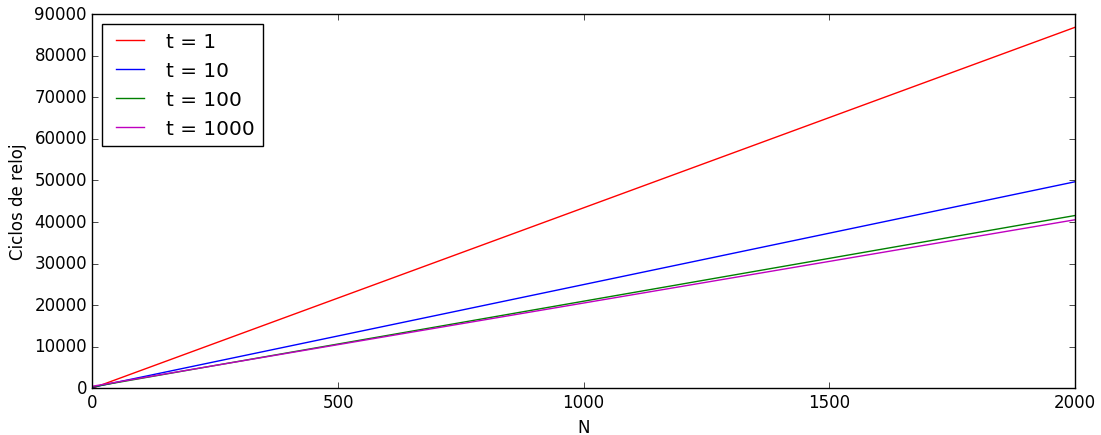
\includegraphics[width=\textwidth]{p2_2_2}
\caption{Comparación entre los ajustes lineales para los diferentes valores de $t$}
\end{figure}

En todos los casos se pudo ajustar satisfactoriamente con una función lineal, como esperábamos a causa de que la complejidad es lineal para todos los casos.

Se observa que cuanto mayor es el valor de $t$, menor es la cantidad de ciclos de reloj necesarias. Esto es así ya que cada una de las genkidamas tiene un rango mayor, lo que resulta en más enemigos muertos por genkidama en promedio. Además se puede observar que el caso con $t$ = 1 está cerca del peor caso (casi 1 $N$ genkidamas) mientras que el caso con $t$ = 1000 está cerca del mejor caso (casi 1 genkidama en total).

\begin{multicols}{2}
Comparando los valores de pendientes ajustadas y el segundo gráfico se puede ver que la pendiente decrece rápidamente al principio, llegando a alcanzar la mitad de su valor. Esto es consistente con la diferencia en complejidad entre el mejor y el peor caso, que es $O(N)$ y $O(2N)$ respectivamente.

\begin{description}
\item[Pendiente para t = 1] $\approx43,416$
\item[Pendiente para t = 10] $\approx24,727$
\item[Pendiente para t = 100] $\approx20,608$
\item[Pendiente para t = 1000] $\approx20,026$
\end{description}
\end{multicols}
%TODO : no es consistente porque antes decia 3N(lo cambie). no se cual poner u,u

\subsubsection{Mediciones con distribución constante y $t$ variable}

Se realizaron mediciones usando siempre la misma distribución generada aleatoriamente con $N$ = 2000 elementos. La separación promedio $d$ entre las coordenadas de los puntos para un caso fue 100, para otro 500 y para otro 1000. Se varió $t$ entre 1 y 2000 y se obtuvieron los siguientes resultados:

\begin{figure}[h!]
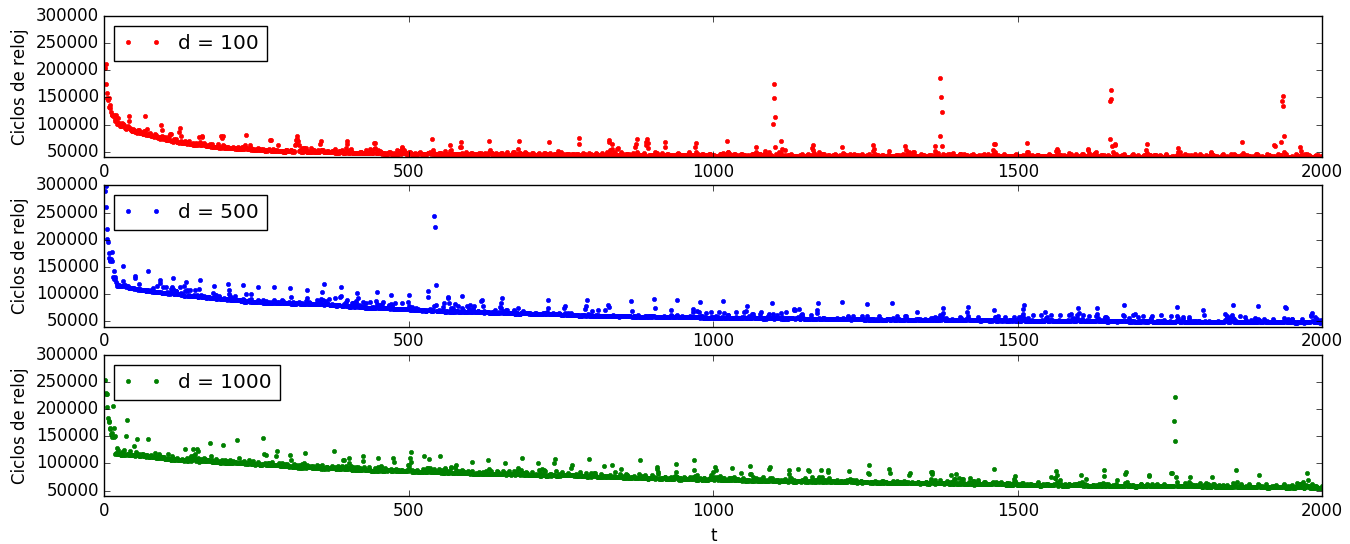
\includegraphics[width=\textwidth]{p2_3}
\caption{Mediciones para $t$ variable y distribución fija con distintas separaciones promedio entre puntos}
\end{figure}

Se observa en todos los casos que cerca de $t$ = 0 la cantidad de ciclos de reloj es alta y desciende abruptamente. También se puede ver que en el caso de los puntos más juntos, se llega al tiempo mínimo (la cota inferior de la cantidad de ciclos de reloj) antes que en los otros dos casos. Esto tiene sentido puesto que el mejor caso debería encontrarse antes cuanto más juntos estén los puntos, cuando $t \approx d$. Y se observa efectivamente que es en esa parte del gráfico en la cual se llega a la asíntota.


\end{document}